\documentclass[fleqn,11pt]{article}

\usepackage[letterpaper,margin=0.75in]{geometry}

\usepackage{amsmath}
\usepackage{booktabs}
\usepackage{graphicx}
\usepackage{listings}

\setlength{\parindent}{1.4em}

\begin{document}

\title{Network Simulation}

\author{Chase Robertson}

\date{20 October 2017}

\maketitle

My test protocol is called transfer.py in the bene/lab2 directory. It can be run with args: -f filename (no default), -l loss (default 0.0), -w window size (default 3000 bytes), and flag -r to enable fast retransmit (default disabled). Two network configuration files were interchanged in transfer.py to model tcp with and without queueing: network.txt and networkWithQueue.txt.

\section{Basic Tests}

A simple network consisting of two nodes and and one bidirectional link was simulated. The bandwidth of the links was set to 10 Mbps, with a propagation delay of 10 milliseconds. Maximum packet size was set to 1,000 bytes.

\begin{enumerate}

\item A test file "test.txt" of 10,000 bytes was sent from n1 to n2 at time 0, with a window size of 3,000 bytes. Different loss rates were tested in each scenario.

\begin{enumerate}
\item Test of 0\% packet loss. This test went as fast as the transmission rate and window size would allow, with no loss to increase delay. \\
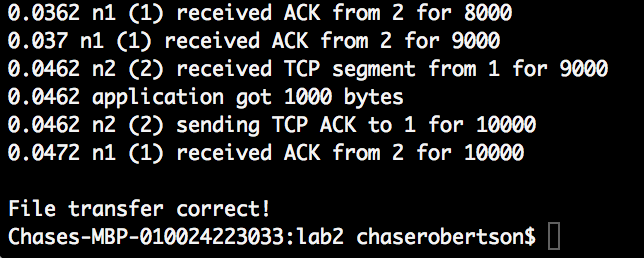
\includegraphics{basic-testtxt0.png}

\item Test of 10\% packet loss. Though this test had only 1 packet lost per 10 sent, the timeout of 1 second ended up increasing total delay by 20 times! \\
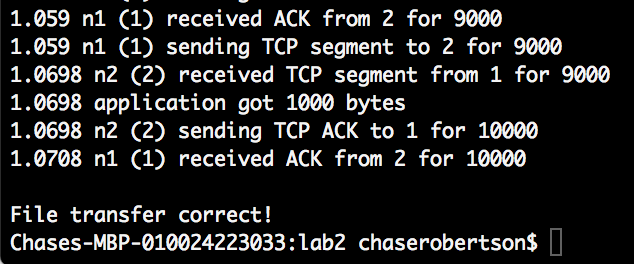
\includegraphics{basic-testtxt10.png}

\item Test of 20\% packet loss. Each packet lost added 1 second of delay waiting for the timeout to signal loss. \\
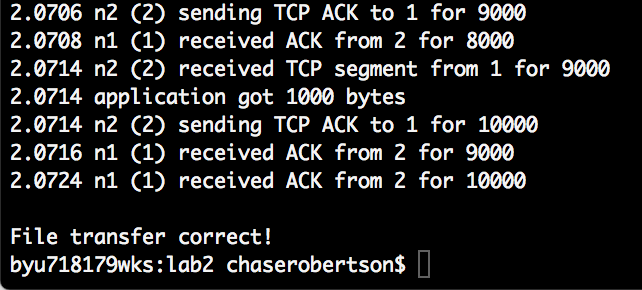
\includegraphics{basic-testtxt20.png}

\item Test of 50\% packet loss. The nature of such heavy packet loss increased the total time of this test far beyond my expectations. Only 10 packets of data ended up causing far more than 5 timeout delays, because each packet lost must be resent, and each resending has its own chance of being lost. \\
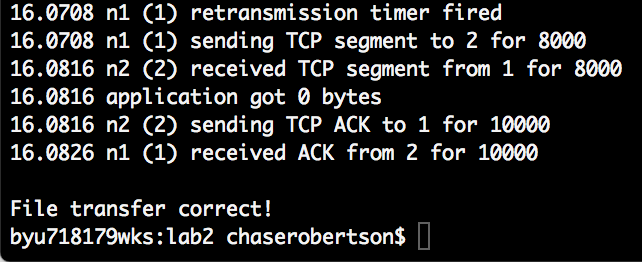
\includegraphics{basic-testtxt50.png}
\end{enumerate}

\item A test file "internet-architecture.pdf" of 514,520 bytes was sent from n1 to n2 at time 0, with a window size of 10,000 bytes. Different loss rates were tested in each scenario.

\begin{enumerate}
\item Test of 0\% packet loss. As expected, total delay of transfer was only limited by transmission speed. \\
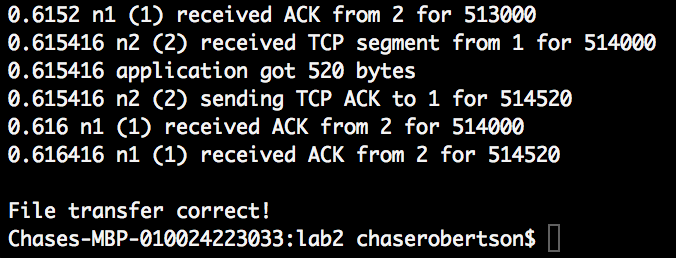
\includegraphics{basic-testpdf0.png}

\item Test of 50\% packet loss. Of the 515 packets of new data sent, 402 were lost. This is because each packet lost must be resent, as well as packets sent after the lost packet, each having its own 50\% chance of also being lost. \\
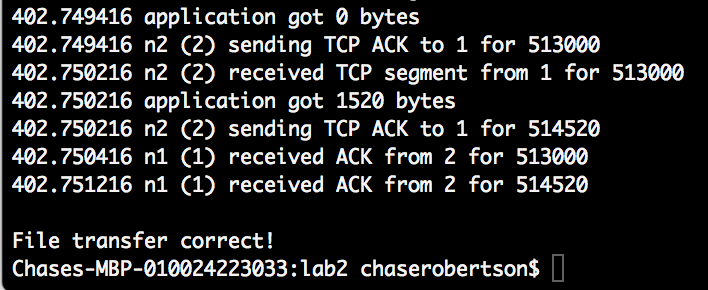
\includegraphics{basic-testpdf50.png}
\end{enumerate}


\end{enumerate}

\section{Fast Retransmit}

The same simple network consisting of two nodes and and one bidirectional link was simulated. The bandwidth of the links was set to 10 Mbps, with a propagation delay of 10 milliseconds. Maximum packet size was set to 1,000 bytes.

\begin{enumerate}
\item A test file "internet-architecture.pdf" of 514,520 bytes was sent from n1 to n2 at time 0, with a window size of 10,000 bytes. The same loss rate of 20\% was tested with and without fast retransmit functionality. My implementation of fast retransmit depended on receiving 4 ACK responses with the same sequence number, then immediately resending the next outstanding packet as though a timeout had occurred.

\begin{enumerate}
\item Test without fast retransmit. Significant delay occurred because it takes a full second to recognize each lost packet. \\
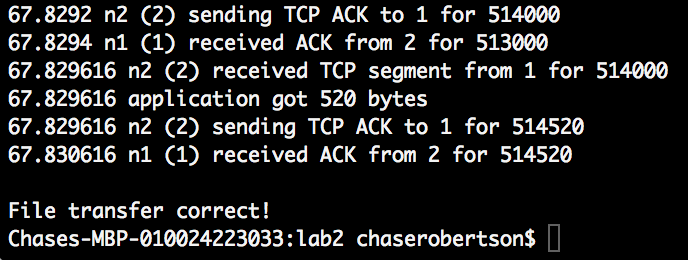
\includegraphics{withoutretransmit.png}

\item Test with fast retransmit. Delay is reduced by a factor of 12, simply by recognizing duplicate cumulative ACK's as a sign of packet loss, thereby short circuiting timeout in most cases. \\
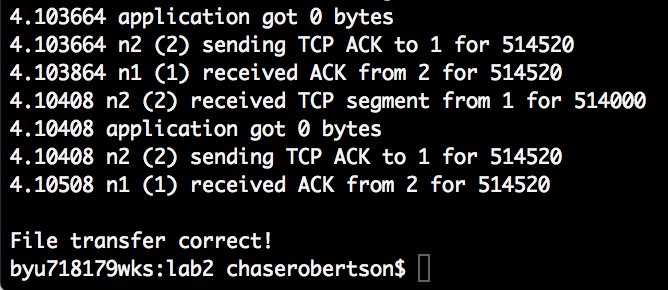
\includegraphics{withretransmit.png}
\end{enumerate}

\end{enumerate}

\section{Experiments}

The same simple network consisting of two nodes and and one bidirectional link was simulated. The bandwidth of the links was set to 10 Mbps, with a propagation delay of 10 milliseconds. Maximum packet size was set to 1,000 bytes. A queue size of 100 was added, and loss rate was set to 0\%. \\
 \\
The throughput of each test transfer was computed as the total bits sent divided by the total time to send the file. The average queueing delay of each test transfer was also calculated (from simulator's queueing log csv file).

\begin{enumerate}
\item A test file "internet-architecture.pdf" of 514,520 bytes was sent from n1 to n2 at time 0, using varying window sizes.

\begin{enumerate}
\item Test with 1,000 byte window size \\
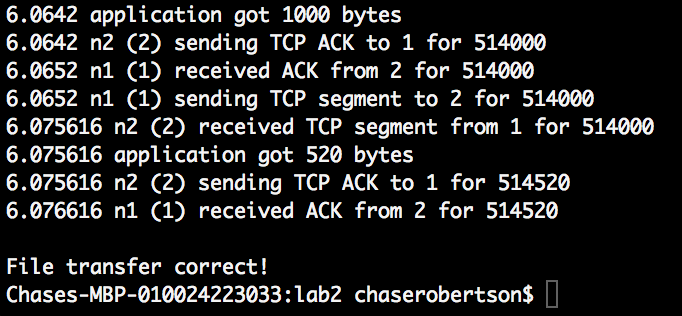
\includegraphics{queue1000.png}

\begin{align*}
throughput &= 4,116,160 bits / 6.0766 sec = 677 Kbps  \\
d_{queue} &= 0 sec
\end{align*}

\item Test with 2,000 byte window size \\
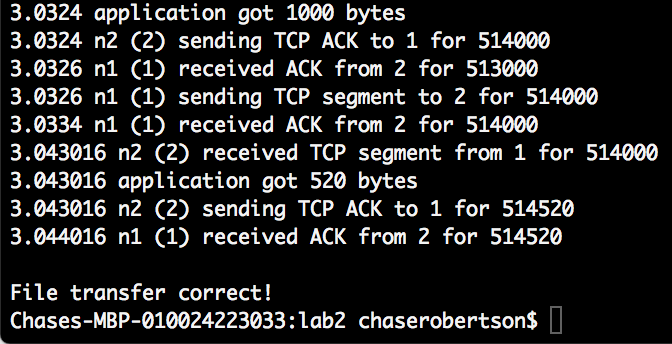
\includegraphics{queue2000.png}

\begin{align*}
throughput &= 4,116,160 bits / 3.044 sec = 1.35 Mbps \\
d_{queue} &= 0.0016 sec
\end{align*}

\item Test with 5,000 byte window size \\
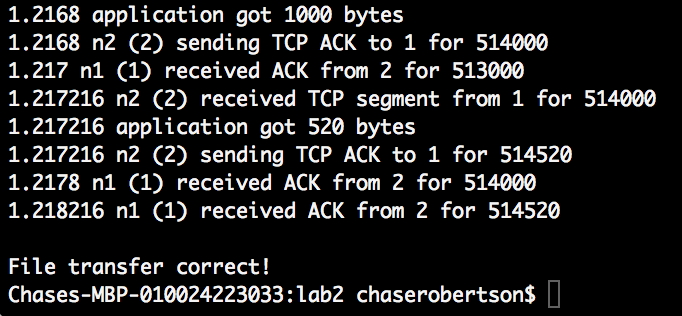
\includegraphics{queue5000.png}

\begin{align*}
throughput &= 4,116,160 / 1.218 = 3.38Mbps \\
d_{queue} &= 0.0136 sec
\end{align*}

\item Test with 10,000 byte window size \\
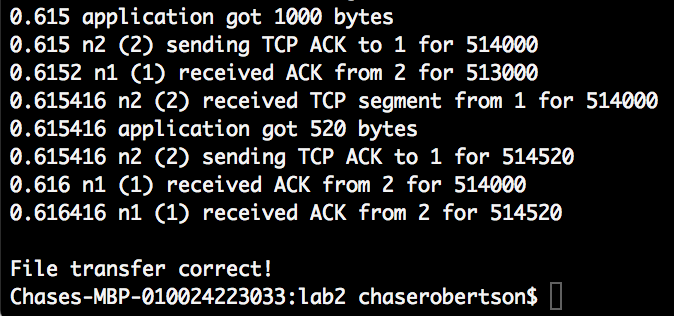
\includegraphics{queue10000.png}

\begin{align*}
throughput &= 4,116,160 / 0.6164 = 6.68Mbps \\
d_{queue} &= 0.032 sec
\end{align*}

\item Test with 15,000 byte window size \\
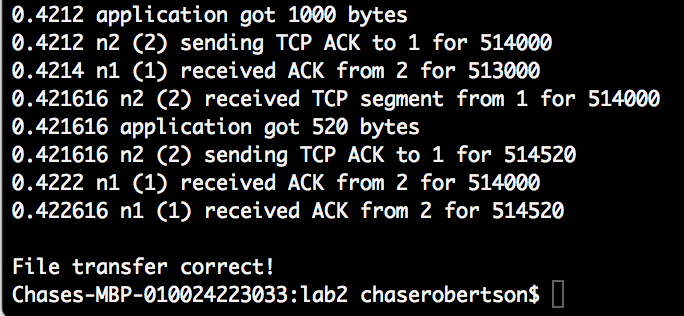
\includegraphics{queue15000.png}

\begin{align*}
throughput &= 4,116,160 / 0.4226 = 9.74Mbps \\
d_{queue} &= 0.412 sec
\end{align*}

\item Test with 20,000 byte window size \\
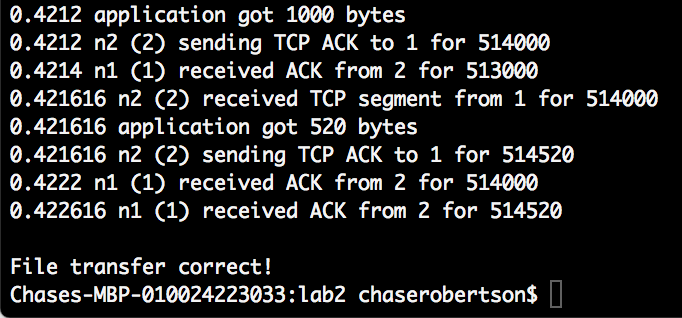
\includegraphics{queue20000.png}

\begin{align*}
throughput &= 4,116,160 / 0.4226 = 9.74Mbps \\
d_{queue} &= 0.420 sec
\end{align*}

\end{enumerate}

\item The throughput and average queueing delay of each test transfer were each plotted as a function of window size.

\begin{enumerate}
\item Throughput vs Window Size \\
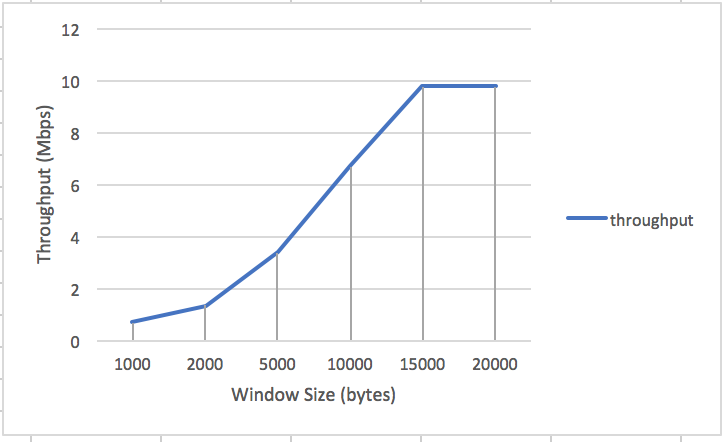
\includegraphics{throughputGraph.png} \\
As window size increases, link utilization also increases because more packets are in transfer at once. Once maximum link utilization is reached, increasing window size doesn't decrease total delay anymore. This can be seen in the difference between total delay time between window sizes 15,000 and 20,000 bytes: there is no difference!

\item Queueing Delay vs Window Size \\
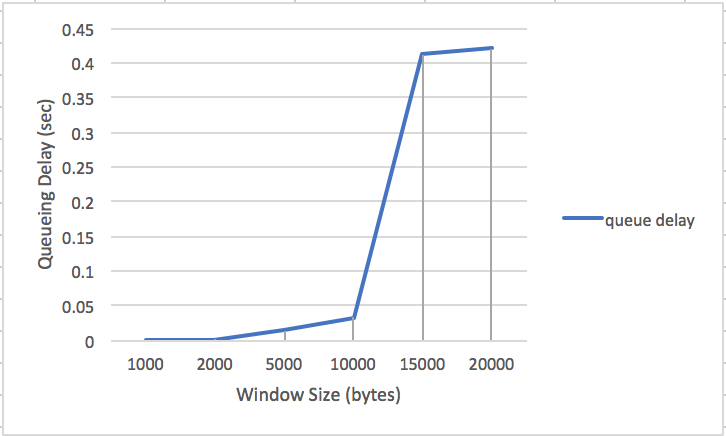
\includegraphics{delayGraph.png} \\
As window size increases, the queue starts to fill with packets and cause some queueing delay. Much more interesting experiments can be conducted with larger window sizes, as the queue fills much more than in these cases. Experiments that include random loss and random packet arrival or readiness would also be more akin to reality.

\end{enumerate}

\end{enumerate}

\end{document}
